\chapter{Administradores, usuarios y personal}
\section{Introducci\'on}
Con frecuencia se suele afirmar, y no es una exageraci\'on (\cite{kn:and94}), 
que el punto m\'as d\'ebil de cualquier sistema
inform\'atico son las personas relacionadas en mayor o menor medida con \'el;
desde un administrador sin una preparaci\'on adecuada o sin la suficiente 
experiencia, hasta un guardia de seguridad que ni siquiera tiene acceso 
l\'ogico al sistema, pero que deja acceder a todo el mundo a la sala de 
operaciones, pasando por supuesto por la gran mayor\'{\i}a de usuarios, que no 
suelen conscientes de que la seguridad tambi\'en les concierne a ellos. Frente 
a cada uno de estos grupos (administradores, usuarios y personal externo al 
sistema) un potencial atacante va a comportarse de una forma determinada para 
conseguir lograr sus objetivos, y sobre cada uno de ellos ha de aplicarse una 
pol\'{\i}tica de seguridad diferente: obviamente podemos exigir a un 
administrador de sistemas unos conocimientos m\'as o menos profundos de temas
relacionados con la seguridad inform\'atica, pero esos conocimientos han de ser
diferentes para el guardia de seguridad (sus conocimientos ser\'{\i}an 
referentes a la seguridad f\'{\i}sica del entorno), y se convierten en simples
nociones b\'asicas si se trata de un usuario medio.\\
\\Hasta ahora hemos hablado de posibles ataques relacionados con el personal de
un sistema inform\'atico; sin embargo, existen otras amenazas a la seguridad
provenientes de ese personal que no son necesariamente ataques en un sentido
estricto de la palabra; en muchos casos no son intencionados, se podr\'{\i}an
catalogar como accidentes, pero el que la amenaza no sea intencionada no implica
que no se deba evitar: decir {\it `no lo hice a prop\'osito'} no va ayudar para 
nada a recuperar unos datos perdidos. En una sala de operaciones, las
personas realizan acciones sobre los sistemas bas\'andose -- en muchos casos
-- \'unicamente en su apreciaci\'on personal de lo que est\'a sucediendo; en
esas circunstancias, dichas acciones pueden ser sorprendentes y devastadoras,
incluso si provienen de los mejores y m\'as cuidadosos administradores 
(\cite{kn:nrc99}).
\section{Ataques potenciales}
\subsection{Ingenier\'{\i}a social}
La ingenier\'{\i}a social consiste en la manipulaci\'on de las personas para
que voluntariamente realicen actos que normalmente no har\'{\i}an 
(\cite{kn:fen99}); aunque a nadie le gusta ser manipulado, en algunos casos no 
es excesivamente perjudicial (por ejemplo un vendedor puede aplicar 
ingenier\'{\i}a social para conocer las necesidades de un cliente y ofrecer 
as\'{\i} mejor sus productos), si las intenciones de quien la pone en 
pr\'actica no son buenas se convierte quiz\'as el m\'etodo de ataque m\'as 
sencillo, menos peligroso para el atacante y por desgracia en uno de los m\'as 
efectivos. Ese atacante puede aprovechar el desconocimiento de unas m\'{\i}nimas
medidas de seguridad por parte de personas relacionadas de una u otra forma
con el sistema para poder enga\~narlas en beneficio propio. Por ejemplo,
imaginemos que un usuario de una m\'aquina Unix recibe el siguiente correo
electr\'onico:
\begin{quote}
\begin{verbatim}
From: Super-User <root@sistema.com>
To: Usuario <user@sistema.com>
Subject: Cambio de clave
Hola,
Para realizar una serie de pruebas orientadas a conseguir un optimo 
funcionamiento de nuestro sistema, es necesario que cambie su clave mediante
la orden 'passwd'. Hasta que reciba un nuevo aviso (aproximadamente en una
semana), por favor, asigne a su contrasenya el valor 'PEPITO' (en 
mayusculas).
Rogamos disculpe las molestias. Saludos,
                        
                                Administrador
\end{verbatim}
\end{quote}
Si el usuario no sabe nada sobre seguridad, es muy probable que siga al pie de
la letra las indicaciones de este {\it e-mail}; pero nadie le asegura que el
correo no haya sido enviado por un atacante -- es muy f\'acil camuflar el 
origen real de un mensaje --, que consigue as\'{\i} un acceso al sistema: no
tiene m\'as que enviar un simple correo, sin complicarse buscando fallos en
los sistemas operativos o la red, para poner en juego toda la seguridad. Sin 
saberlo, y encima pensando que lo hace por el bien com\'un, el usuario est\'a 
ayudando al pirata a romper todo el esquema de seguridad de nuestra m\'aquina.\\
\\Pero no siempre el atacante se aprovecha de la buena fe de los usuarios para
lograr sus prop\'ositos; tampoco es extra\~no que intente enga\~nar al 
propio administrador del sistema\footnote{Esto simplemente es para dar m\'as
credibilidad, pero no es necesario que el usuario real no haya conectado en
mucho tiempo.}. Por ejemplo, imaginemos que la m\'aquina
tiene el puerto {\it finger} abierto, y el atacante detecta un nombre de 
usuario que nunca ha conectado al sistema; en este caso, una simple llamada 
telef\'onica puede bastarle para conseguir el acceso:
\tt
\begin{quote}
$[$Administrador$]$ Buenos dias, aqu\'{\i} \'area de sistemas, en qu\'e 
podemos\\
ayudarle?\\
$[$Atacante$]$ Hola, soy Jos\'e Luis P\'erez, llamaba porque no consigo\\
recordar mi {\it password} en la m\'aquina {\it sistema.upv.es}.\\
$[$Administrador$]$ Un momento, me puede decir su nombre de usuario?\\
$[$Atacante$]$ S\'{\i}, claro, es jlperez.\\
$[$Administrador$]$ Muy bien, la nueva contrase\~na que acabo de asignarle\\
es {\it rudolf}. Por favor, nada m\'as conectar, no olvide cambiarla.\\
$[$Atacante$]$ Por supuesto. Muchas gracias, ha sido muy amable.\\
$[$Administrador$]$ De nada, un saludo.
\end{quote}
\rm
Como podemos ver, estamos en la situaci\'on opuesta a la anterior: ahora es
el {\it root} quien facilita la entrada del atacante en la m\'aquina; lo \'unico
que este ha necesitado es un nombre de usuario v\'alido.\\
\\Evidentemente, cualquier mensaje, llamada telef\'onica o similar que un 
usuario reciba debe ser puesto inmediatamente en conocimiento del administrador
del sistema; hay que recordar a los usuarios que en ning\'un caso se necesita 
su contrase\~na para realizar tareas administrativas en la m\'aquina. De la
misma forma, si es el administrador quien directamente recibe algo parecido a
lo que acabamos de ver, quiz\'as sea conveniente notificar el hecho a los
responsables de la organizaci\'on, y por supuesto poner la m\'axima atenci\'on
en la seguridad de los sistemas involucrados, ya que en este caso se sabe a
ciencia cierta que alguien intenta comprometer nuestra seguridad; en 
\cite{kn:rad97} y \cite{kn:win95} se muestran algunas de las reglas b\'asicas 
que debemos 
seguir en nuestra organizaci\'on para prevenir ataques de ingenier\'{\i}a social
y tambi\'en para, en el caso de que se produzcan, reducir al m\'{\i}nimo sus
efectos.
\subsection{{\it Shoulder Surfing}} 
Otro tipo de ataque relacionado con la ingenuidad de los usuarios del sistema 
(pero tambi\'en con el control de acceso f\'{\i}sico)
es el denominado {\it shoulder surfing}. Consiste en `espiar' f\'{\i}sicamente
a los usuarios, para obtener generalmente claves de acceso al sistema. Por
ejemplo, una medida que lamentablemente utilizan muchos usuarios para recordar
sus contrase\~nas es apuntarlas en un papel pegado al monitor de su PC o 
escribirlas en la parte de abajo del teclado; cualquiera que pase por delante 
del puesto de trabajo, sin problemas puede leer el {\it login}, {\it password}
e incluso el nombre de m\'aquina a la que pertenecen. Esto, que nos puede 
parecer una gran tonter\'{\i}a, por desgracia no lo es, y se utiliza m\'as de
lo que muchos administradores o responsables de seguridad piensan; y no s\'olo
en entornos `privados' o con un control de acceso restringido, como pueda ser
una sala de operaciones de un centro de c\'alculo, sino en lugares a los que
cualquiera puede llegar sin ninguna acreditaci\'on: personalmente, hace unos 
a\~nos pude leer claramente {\it `post-it'} pegados a los monitores de los PCs 
utilizados por el personal de informaci\'on de unos grandes almacenes de 
Valencia, en los que aparec\'{\i}an el nombre de usuario, la clave y el 
tel\'efono de
varios sistemas de la empresa; cualquiera que se acercase al mostrador 
pod\'{\i}a leer y memorizar esta informaci\'on sin problemas.\\
\\El {\it shoulder surfing} no siempre se ve beneficiado por la ingenuidad de 
los simples usuarios de un equipo; en determinadas ocasiones son los propios
programadores (gente que te\'oricamente ha de saber algo m\'as sobre seguridad
que el personal de administraci\'on o de atenci\'on al p\'ublico) los que 
dise\~nan aplicaciones muy susceptibles de sufrir ataques de este tipo. Por
ejemplo, en ciertas aplicaciones -- especialmente algunas que se ejecutan 
sobre MS Windows, y que son m\'as o menos antiguas -- muestran claramente en 
pantalla las contrase\~nas al ser 
tecleadas. Cualquiera situado cerca de una persona que las est\'a utilizando
puede leer claramente esa clave; un perfecto ejemplo de lo que {\sc no} se 
debe hacer nunca.
\subsection{Masquerading}
El ataque denominado de {\it masquerading} o mascarada consiste simplemente en
suplantar la identidad de cierto usuario autorizado de un sistema inform\'atico
o su entorno; esta suplantaci\'on puede realizarse electr\'onicamente -- un 
usuario utiliza para acceder a una m\'aquina un {\it login} y {\it password} 
que no le pertenecen -- o en persona. En este punto hablaremos brevemente de
este \'ultimo caso, la suplantaci\'on en persona, un ataque relativo tanto a
la seguridad f\'{\i}sica del entorno de operaciones como a la seguridad del
personal.\\
\\La mascarada no es un ataque habitual en entornos normales; en estos, o bien
existen \'areas de acceso semip\'ublico, donde un atacante no tiene que hacer
nada especial para conseguir acceso -- y por tanto no cabe hablar de {\it
masquerading} -- o bien \'areas de acceso restringido pero controlado por el
propio personal de la organizaci\'on, como despachos o laboratorios. En este
caso un ataque v\'{\i}a mascarada no suele ser efectivo, ya que es muy f\'acil
detectar al intruso (otro tema ser\'{\i}a si realmente se toma alguna medida al
detectarlo o simplemente se le deja seguir, ah\'{\i} ya entrar\'{\i}a en
juego la formaci\'on de los usuarios) por tratarse de \'areas dentro de las 
cuales todo el personal `habitual' se conoce. El {\it masquerading} es m\'as
habitual en entornos donde existen controles de acceso f\'{\i}sico, y donde
un intruso puede `enga\~nar' al dispositivo -- o persona -- que realiza el 
control, por ejemplo con una tarjeta de identificaci\'on robada que un lector
acepta o con un carn\'e falsificado que un guardia de seguridad da por bueno.\\ 
\\Una variante del {\it masquerading} lo constituye el ataque denominado {\it
piggybacking}, que consiste simplemente en seguir a un usuario autorizado hasta
un \'area restringida y acceder a la misma gracias a la autorizaci\'on otorgada
a dicho usuario. Contra esto se deben aplicar las mismas medidas que contra
la mascarada f\'{\i}sica: controles de acceso estrictos, y convenientemente 
verificados. Los ejemplos de {\it piggybacking} son muy habituales: desde un
atacante que se viste con un mono de trabajo y que carga con un pesado equipo 
inform\'atico en la puerta de una sala de operaciones, para que justo cuando
un usuario autorizado llegue le abra dicha puerta y le permita el acceso por 
delante del guardia de seguridad, hasta la cl\'asica an\'ecdota que todos los
auditores explican como suya, sobre el reconocedor de tarjetas inteligentes que
abre la puerta de una sala pero que una vez abierta no se preocupa en contar
cuantas personas la atraviesan, podr\'{\i}amos estar durante d\'{\i}as dando
ejemplos de ataques exitosos utilizando la t\'ecnica del {\it piggybacking}.
\subsection{Basureo}
La t\'ecnica del basureo (en ingl\'es, {\it scavenging}) est\'a relacionada
tanto con los usuarios como con la seguridad f\'{\i}sica de los sistemas, de la
que hemos hablado en el anterior cap\'{\i}tulo; consiste en obtener 
informaci\'on dejada en o alrededor de un sistema inform\'atico tras la 
ejecuci\'on de un trabajo (\cite{kn:par81}). El basureo puede ser f\'{\i}sico,
como buscar en cubos de basura ({\it trashing}, traducido tambi\'en por
{\it basureo}) listados de impresi\'on o copias de documentos, o l\'ogico, como
analizar {\it buffers} de impresoras, memoria liberada por procesos, o bloques
de un disco que el sistema acaba de marcar como libres, en busca de 
informaci\'on.\\
\\Aunque esta t\'ecnica no es muy utilizada en la mayor\'{\i}a de entornos, 
hemos de pensar
que si un usuario tira a la basura documentos que proporcionen informaci\'on 
sobre nuestro sistema, cualquier potencial atacante puede aprovechar esa 
informaci\'on para conseguir acceder al equipo; algo tan simple como una 
factura en la que se especifiquen n\'umeros de tel\'efono o nombres (reales o
de entrada al sistema) de usuarios puede convertirse en una valiosa 
informaci\'on para un atacante. Adem\'as, en ocasiones ni siquiera es necesario
andar revolviendo por los cubos de basura en busca de informaci\'on 
comprometedora: la carencia de nociones b\'asicas sobre seguridad inform\'atica
hace posible que los usuarios dejen al alcance de cualquiera informaci\'on
vital de cara a mantener un sistema seguro. Personalmente, en un aula de
inform\'atica de la Universidad Polit\'ecnica de Valencia encontr\'e por 
casualidad una hoja de papel
que estaba siendo utilizada a modo de alfombrilla para el rat\'on; esta hoja
era una carta personalizada que el director de la Escuela T\'ecnica Superior
de Ingenieros Industriales hab\'{\i}a enviado a cada alumno de esa escuela 
para informarles de sus nuevas claves de acceso a ciertos recursos de la
universidad, ya que las anteriores hab\'{\i}an tenido que ser cambiadas porque 
un pirata las captur\'o. Con esa sencilla hoja de papel (en la figura 
\ref{scav} se muestra una copia -- con los datos importantes ocultos, en
el original no hay nada `censurado' --) cualquiera podr\'{\i}a haber le\'{\i}do
el correo de ese usuario, utilizar su acceso remoto de la universidad, 
curiosear en su expediente o participar en foros de asignaturas bajo la 
identidad del usuario atacado.\\
\begin{figure}
\begin{center}
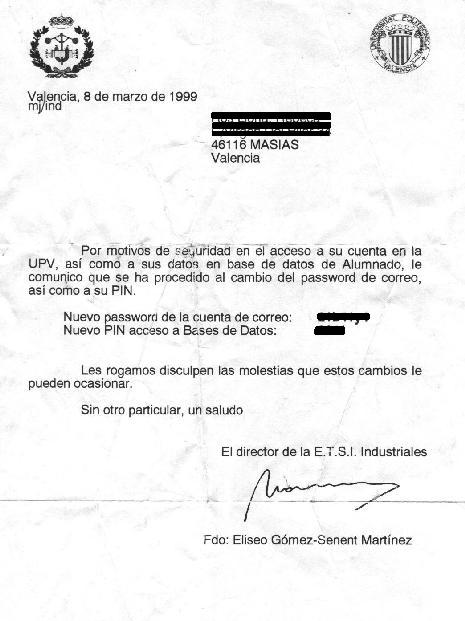
\includegraphics[width=\textwidth]{scav.png}
\caption{El resultado de un basureo involuntario.}
\label{scav}
\end{center}
\end{figure}
\\Como hemos dicho el basureo no es un ataque habitual en organizaciones
`normales', simplemente porque los datos con los que estan trabajan no suelen 
ser de alta confidencialidad. De cualquier forma, si deseamos evitar problemas 
lo m\'as inmediato es utilizar una m\'aquina trituradora de papel (su precio no 
suele ser prohibitivo, y la inversi\'on quiz\'as valga la pena) para destruir 
toda la 
documentaci\'on antes de arrojarla a la basura; incluso nos puede interesar
contratar los servicios de compa\~n\'{\i}as dedicadas exclusivamente a la
destrucci\'on de estos soportes. En el caso de sistemas de almacenamiento 
l\'ogico (discos, CD-ROMs, cintas\ldots) tambi\'en es importante una correcta
inutilizaci\'on de los mismos para que un potencial atacante no pueda extraer
informaci\'on comprometedora; no suele ser suficiente el simple borrado del
medio o un leve da\~no f\'{\i}sico (por ejemplo, partir un CD-ROM), ya que como 
comentaremos al hablar de
recuperaci\'on de datos existen empresas capaces de extraer hasta el \'ultimo
{\it bit} de un medio borrado o da\~nado. Lo m\'as efectivo ser\'{\i}a un
borrado seguro, seguido de una destrucci\'on f\'{\i}sica importante que haga
imposible la reconstrucci\'on del medio.
\subsection{Actos delictivos}
Bajo este nombre englobamos actos tipificados claramente como delitos por las
leyes espa\~nolas, como el chantaje, el soborno o la amenaza. Esto no implica
que el resto de actividades no sean (o deban ser) delitos, sino simplemente que
en la pr\'actica a nadie se le castiga `legalmente' por pasear por una sala
de operaciones en busca de claves apuntadas en teclados, pero s\'{\i} que se
le puede castigar por amenazar a un operador para que le permita el acceso al
sistema.\\
\\Por suerte, la naturaleza de la informaci\'on con la que se trabaja en la
mayor parte de
entornos hace poco probable que alguien amenaze o chantajee a un operador
para conseguir ciertos datos; al tratarse de informaci\'on poco sensible, 
en la mayor\'{\i}a de situaciones los atacantes no llegan a estos extremos para
acceder al sistema, sino que utilizan procedimientos menos arriesgados como la
ingenier\'{\i}a social o la captura de datos que viajan por la red. No obstante,
si en alguna ocasi\'on nos encontramos en estas situaciones, siempre es 
conveniente la denuncia; aunque en principio podamos ceder ante las presiones 
de un delincuente, hemos de tener presente que si mostramos cierta debilidad, 
una vez que \'este consiga sus prop\'ositos nada le va a impedir seguir 
amenaz\'andonos o chantaje\'andonos para obtener m\'as informaci\'on. Si 
actuamos con la suficiente discrecci\'on, las autoridades pueden f\'acilmente
llevar al individuo ante la justicia sin necesidad de grandes esc\'andalos que
pueden afectar gravemente a la imagen de nuestra organizaci\'on.
\section{>Qu\'e hacer ante estos problemas?}
La soluci\'on a problemas relacionados con el personal es con frecuencia mucho
m\'as compleja que la de problemas de seguridad l\'ogica o seguridad de la
red: mientras que un administrador puede aprovechar herramientas de seguridad, 
capacidades del sistema operativo, o cifrado de datos para prevenir ciertos 
ataques, es mucho m\'as dif\'{\i}cil para \'el concienciar a los usuarios de 
unas m\'{\i}nimas medidas de prevenci\'on o convencer a un guardia de seguridad
de que s\'olo deje acceder a la sala de operaciones a un n\'umero restringido de
personas.\\
\\Generalmente los usuarios de m\'aquinas Unix en entornos habituales son 
personas
muy poco formadas en el manejo del sistema operativo, y mucho menos en lo que
a seguridad inform\'atica se refiere; se suele tratar de usuarios que 
s\'olo utilizan la m\'aquina para ejecutar aplicaciones muy concretas 
(simulaciones, compiladores, gesti\'on del correo electr\'onico, aplicaciones 
cient\'{\i}ficas\ldots relacionadas con su \'area de trabajo), y cuya \'unica 
preocupaci\'on es que sus datos est\'en listos cuando
los requieren, de la forma m\'as f\'acil y r\'apida posible. Incluso el 
administrador de ciertos sistemas es uno de estos usuarios, elegido dentro del
grupo (o mucho peor, son todos los usuarios). Evidentemente, resulta muy 
dif\'{\i}cil concienciar a estas personas de la necesidad de seguridad en el
entorno; posturas como {\it `no importa que mi clave sea d\'ebil, s\'olo
utilizo la cuenta para imprimir con la l\'aser'} son por desgracia demasiado
frecuentes. El responsable de seguridad ha de concienciar a todas estas personas
de la necesidad de la seguridad para que el entorno de trabajo funcione como
se espera de \'el; la seguridad inform\'atica se ha de ver como una cadena que
se rompe si falla uno de sus eslabones: no importa que tengamos un sistema 
de cifrado resistente a cualquier ataque o una autenticaci\'on fuerte de 
cualquier entidad del sistema si un intruso es capaz de obtener un nombre de 
usuario con su correspondiente contrase\~na simplemente llamando por tel\'efono
a una secretaria.\\
\\Adem\'as de concienciaci\'on de los usuarios y administradores en cuanto
a seguridad se refiere (esto ser\'{\i}a el {\sc qu\'e}), para conseguir un 
sistema fiable es necesaria la {\bf formaci\'on} de los mismos (el {\sc 
c\'omo}). De la misma forma que a nadie se le ocurre conducir sin tener unos
conocimientos b\'asicos sobre un autom\'ovil, no deber\'{\i}a ser tan habitual
que la gente utilice o administre Unix sin unos conocimientos previos del
sistema operativo. Evidentemente, a un qu\'{\i}mico que utiliza el sistema para
simular el comportamiento de determinada sustancia bajo ciertas condiciones no
se le puede exigir un curso intensivo o unos grandes conocimientos de mecanismos
de seguridad en Unix; pero s\'{\i} que ser\'{\i}a recomendable que conozca
unas ideas b\'asicas (volviendo al ejemplo del autom\'ovil, para conducir un
coche a nadie se le exige ser un as de la mec\'anica, pero s\'{\i} unas 
cualidades m\'{\i}nimas). Estas ideas b\'asicas se pueden incluso resumir en una
hoja que se le entregue a cada usuario al darlos de alta en el sistema. Si
pasamos a hablar de administradores, s\'{\i} que ser\'{\i}a recomendable 
exigirles un cierto nivel de conocimientos de seguridad, nivel que se puede 
adquirir simplemente leyendo alg\'un libro (especialmente recomendado 
ser\'{\i}a \cite{kn:spa96} o, para los que dispongan de menos tiempo, 
\cite{kn:rcg96}).\\
\\Un grupo de personas m\'as delicado si cabe es el conjunto formado por todos
aquellos que no son usuarios del sistema pero que en cierta forma pueden llegar 
a comprometerlo. Por ejemplo, en este conjunto encontramos elementos tan 
diversos como guardias de seguridad que controlen el acceso a las instalaciones 
inform\'aticas o personal de administraci\'on y servicios que no utilicen el 
sistema pero que tengan acceso f\'{\i}sico a \'el, como electricistas, bedeles
o personal de limpieza. Sin entrar en temas que seguramente no son aplicables
a los sistemas habituales, como el espionaje industrial o el terrorismo
de alta magnitud\footnote{Temas que habr\'{\i}a que tener en cuenta en otro
tipo de redes.}, simplemente hemos de concienciar y ense\~nar a estos `usuarios'
unas medidas b\'asicas a tomar para no poner en peligro nuestra seguridad;
estas medidas dependen por supuesto de la funci\'on de cada unas personas 
realice.\\
\\Pero, >qu\'e sucede cuando el personal de nuestra propia organizaci\'on 
produce ataques (y no accidentes) sobre nuestros sistemas? En este caso las
consecuencias pueden ser grav\'{\i}simas, y por tanto las medidad de 
protecci\'on y detecci\'on han de ser estrictas. Se ha de llevar a cabo un 
control estricto de las actividades que se realizan en la organizaci\'on, por
ejemplo mediante pol\'{\i}ticas que han de ser de obligado cumplimiento, 
as\'{\i} como un control de acceso a todos los recursos de los que disponemos
(mediante mecanismos de autenticaci\'on de usuarios, alarmas, etc.). Adem\'as,
las sanciones en caso de incumplimiento de las normas han de ser efectivas y
ejemplares: si un usuario viola intencionadamente nuestra seguridad y no se
le sanciona adecuadamente, estamos invitando al resto de usuarios a que hagan
lo mismo. En el punto siguiente vamos a hablar con m\'as profundidad de estos 
atacantes, denominados {\bf internos}.
\section{El atacante interno}
En el punto anterior hemos presentado al personal de nuestra organizaci\'on
como v\'{\i}ctima de los ataques realizados por agentes externos a la misma;
sin embargo, 
seg\'un \cite{kn:cow92} el 80\% de los fraudes, robos, sabotajes o accidentes
relacionados con los sistemas inform\'aticos son causados por el propio personal
de la organizaci\'on propietaria de dichos sistemas, lo que se suele denominar
el {\it insider factor}. >Qu\'e significa esto? 
Principalmente que la mayor amenaza a nuestros equipos viene de parte de
personas que han trabajado o trabajan con los mismos. Esto, que es realmente
preocupante, lo es mucho m\'as si analizamos la situaci\'on con un m\'{\i}nimo
de detalle: una persona que trabaje codo a codo con el administrador, el
programador, o el responsable de seguridad de una m\'aquina conoce perfectamente
el sistema, sus barreras, sus puntos d\'ebiles\ldots de forma que un ataque
realizado por esa persona va a ser much\'{\i}simo m\'as directo, dif\'{\i}cil
de detectar, y sobre todo, efectivo, que el que un atacante externo (que 
necesita recopilar informaci\'on, intentar probar fallos de seguridad o 
conseguir privilegios) pueda ejecutar.\\
\\Pero, >por qu\'e va a querer alguien atacar a su propia organizaci\'on? >Por
qu\'e alguien va a arriesgarse a perder su trabajo, romper su carrera o incluso 
a ir a la
c\'arcel? Como se acostumbra a decir, todos tenemos un precio; no importa lo
honestos que seamos o que queramos creer que somos: dinero, chantaje, factores
psicol\'ogicos\ldots nos pueden arrastrar a vender informaci\'on, a robar
ficheros o simplemente a proporcionar acceso a terceros que se encarguen del
trabajo sucio. En una empresa, un empleado puede considerarse mal pagado e 
intentar conseguir un sueldo extra a base de vender informaci\'on; en un banco,
alguien que a diario trabaje con los sistemas inform\'aticos puede darse
cuenta de la facilidad para desviar fondos a una cuenta sin levantar sospechas;
en una base militar, un pa\'{\i}s enemigo puede secuestrar a la mujer de un
administrador para que \'este les pase informaci\'on confidencial. Existen
numerosos estudios (\cite{kn:syk70}, \cite{kn:cor86}, \cite{kn:hol83}, 
\cite{kn:kat88}, \cite{kn:rei89}\ldots) que tratan de explicar los motivos que 
llevan a una persona a cometer delitos, inform\'aticos o no, contra su propia 
organizaci\'on, pero sea cual sea el motivo la cuesti\'on est\'a en que tales
ataques existen, son numerosos, y hay que tomar medidas contra ellos.\\
\\>C\'omo prevenir o defendernos de los atacantes internos? En una
empresa, una norma b\'asica ser\'{\i}a verificar el {\it curriculum} de
cualquier aspirante a nuevo miembro (no simplemente leerlo y darlo por bueno,
sino comprobar los datos y directamente descartar al aspirante si se detecta
una mentira); si buscamos algo m\'as de seguridad -- por ejemplo, sistemas
militares -- tambi\'en es recomendable investigar el pasado de cada aspirante
a pertenecer a la organizaci\'on, buscando sobre todo espacios en blanco durante
los que no se sabe muy bien qu\'e ha hecho o a qu\'e se ha dedicado esa
persona (>qui\'en nos asegura que ese par\'entesis de tres a\~nos durante los
que el aspirante asegura que estuvo trabajando para una empresa extranjera no
los pas\'o realmente en la carcel por delitos inform\'aticos?). Si siguiendo
ejemplos como estos podemos asegurar la integridad de todos los que entran
a formar parte del equipo, habremos dado un importante paso en la prevenci\'on
de ataques internos.\\
\\Tampoco debemos olvidar que el hecho de que alguien entre `limpio' a nuestra
organizaci\'on no implica que vaya a seguir as\'{\i} durante el tiempo que
trabaje para nosotros, y mucho menos cuando abandone su trabajo. Para minimizar
el da\~no que un atacante interno nos puede causar se suelen seguir unos
principios fundamentales (\cite{kn:smi92}, \cite{kn:spa96}, 
\cite{kn:pla83}\ldots) que se aplican sobre el personal de la empresa:
\begin{itemize}
\item {\bf Necesidad de saber} ({\it Need to know}) o m\'{\i}nimo privilegio\\
A cada usuario se le debe otorgar el m\'{\i}nimo privilegio que necesite para
desepe\~nar correctamente su funci\'on, es decir, se le debe permitir que
sepa s\'olamente lo que necesita para trabajar. De esta forma, un programador
no tiene por qu\'e conocer las pol\'{\i}ticas de copia de seguridad de la
m\'aquina, ni un alumno tiene que poseer privilegios en un sistema de
pr\'acticas.
\item {\bf Conocimiento parcial} ({\it Dual Control})\\
Las actividades m\'as delicadas dentro de la organizaci\'on en cuanto a
seguridad se refiere (por ejemplo, el conocimiento de la clave de {\it root} de
una m\'aquina) deben ser realizadas por dos personas competentes, de forma que
si uno de ellos comete un error o intenta violar las pol\'{\i}ticas de
seguridad el otro pueda darse cuenta r\'apidamente y subsanarlo o evitarlo. De
la misma forma, aplicar este principio asegura que si uno de los responsables
abandona la organizaci\'on o tiene un accidente el otro pueda seguir operando
los sistemas mientras una nueva persona sustituye a su compa\~nero.
\item {\bf Rotaci\'on de funciones}\\
Quiz\'as la mayor amenaza al conocimiento parcial es la potencial complicidad que
los dos responsables de cierta tarea puedan llegar a establecer, de forma que
entre los dos sean capaces de ocultar las violaciones de seguridad que nuestros
sistemas puedan sufrir; incluso puede
suceder lo contrario: que ambas personas sean enemigos y esto repercuta en
el buen funcionamiento de la pol\'{\i}tica de seguridad establecida. Para evitar
ambos problemas, una norma com\'un es rotar -- siempre dentro de unos
l\'{\i}mites -- a las personas a lo largo de diferentes responsabilidades, de
forma que a la larga todos puedan vigilar a todos; esto tambi\'en es muy
\'util en caso de que alguno de los responsables abandone la organizaci\'on, ya
que en este caso sus tareas ser\'an cubiertas m\'as r\'apidamente.
\item {\bf Separaci\'on de funciones}\\
No es en absoluto recomendable que una sola persona (o dos, si establecemos un
control dual) posea o posean demasiada 
informaci\'on sobre la seguridad de la organizaci\'on; es necesario que se 
definan y separen correctamente las funciones de cada persona, de forma que
alguien cuya tarea es velar por la seguridad de un sistema no posea \'el mismo
la capacidad para violar dicha seguridad sin que nadie se percate de ello.
\end{itemize} 
Si aplicamos correctamente los principios anteriores en nuestra pol\'{\i}tica
de personal vamos a evitar muchos problemas de seguridad, no s\'olo cuando
un usuario trabaja para nuestro entorno sino lo que es igual de importante,
cuando abandona la organizaci\'on. Cuando esto sucede se debe cancelar {\bf
inmediatamente} el acceso de esa persona a todos nuestros recursos (cuentas de
usuario, servicio de acceso remoto, unidades de red\ldots), y tambi\'en 
cambiar las claves que ese usuario conoc\'{\i}a. Especialmente en los entornos 
de I+D quiz\'as
esto es algo complicado debido a la gran movilidad de usuarios (un profesor
invitado durante un mes a la universidad, un proyectando que s\'olo necesita
acceso a una m\'aquina mientras que realiza su proyecto\ldots), por lo que es
aqu\'{\i} donde se suelen ver mayores barbaridades en los sistemas: desde 
cuentas que hace a\~nos que no se utilizan hasta direcciones de correo de gente
que dej\'o de trabajar para la organizaci\'on hace a\~nos. Evidentemente, este
tipo de cosas son muy preocupantes para la seguridad, y es justo en estos
accesos no utilizados donde un atacante puede encontrar una de las mejores 
puertas de entrada a los sistemas: simplemente hemos de pensar que si el usuario
de una cuenta hace a\~nos que no la utiliza, por l\'ogica hace a\~nos que esa
clave no se cambia.\\
\\Hasta ahora hemos hablado principalmente de los problemas que nos pueden causar
las personas que trabajan para la organizaci\'on; no obstante, las redes de I+D 
son bastante peculiares a la hora de hablar de ataques internos. Se trata de 
sistemas en los que un elevado n\'umero de usuarios -- los alumnos -- puede
considerar un reto personal o intelectual (?) saltarse las medidas de 
protecci\'on impuestas en la red; adem\'as, y especialmente en universidades
t\'ecnicas, por la naturaleza de sus 
estudios muchos alumnos llegan a poseer elevados conocimientos sobre sistemas
operativos y redes, lo que evidentemente es un riesgo a\~nadido: no es lo mismo
proteger de ataques internos una m\'aquina Unix en una Facultad de Derecho, 
donde {\it a priori} muy pocos alumnos tendr\'an el inter\'es o los 
conocimientos suficientes para saltarse la seguridad del sistema, que en una 
Facultad de Inform\'atica, donde el que m\'as y el que menos tiene nociones de 
seguridad o de Unix y a diario se trabaja en estos entornos.\\
\\Las normas vistas aqu\'{\i} seguramente se pueden aplicar sobre el 
personal de la organizaci\'on, pero no sobre los alumnos (que es justamente
de quienes provienen la mayor\'{\i}a de ataques): no podemos obligar a un
alumno de nuevo ingreso a que nos muestre un resumen de su vida, ni mucho menos
tenemos capacidad para verificar los datos de treinta o cincuenta mil alumnos.
Incluso si pudi\'eramos, >ser\'{\i}a legal o \'etico denegar el acceso a la
universidad a alguien con antecedentes penales, por ejemplo? Seguramente 
no\ldots De esta forma, en organismos de I+D nos debemos ce\~nir a otros
mecanismos de prevenci\'on, por ejemplo en forma de sanciones ejemplares para
todos aquellos que utilicen los recursos del centro para cometer delitos
inform\'aticos; sin llegar a los tribunales, las posibles penas
impuestas dentro de la universidad son a veces m\'as efectivas que una denuncia
en el juzgado, donde los piratas incluso despiertan cierta simpat\'{\i}a entre 
muchos abogados y jueces.
